%\documentclass[danish,12pt,a4paper]{report}
\documentclass[danish,12pt,a4paper]{report}

\usepackage[utf8]{inputenc}					
\usepackage[danish]{babel}				% Dokumentets sprog
\usepackage[T1]{fontenc}		
\usepackage{amsmath,amsthm,amssymb,amsfonts,bm}
\usepackage{ragged2e,anyfontsize}
\usepackage{etex}
\usepackage[titletoc]{appendix}
\usepackage{thmtools}
\usepackage[makeroom]{cancel}
\usepackage{placeins}
\usepackage{multirow}
\usepackage{mathtools}
\usepackage[danish]{varioref}
\usepackage[numbers]{natbib}
\usepackage{dirtytalk}
\usepackage{blindtext}
\RequirePackage{etex}
\usepackage{graphicx}
\usepackage{flafter}
\usepackage{float}
\usepackage{lastpage}
\usepackage{fancyhdr}
\usepackage{etoolbox}
\usepackage{mdframed}
\usepackage{enumitem}
\usepackage[a4paper]{geometry}
\usepackage{a4wide}
\usepackage{parskip}
\usepackage{booktabs}
\usepackage{rotating}
\usepackage{colortbl}
\usepackage{textcomp}
\usepackage{tabularx}
\usepackage{url}
\usepackage{hyperref}
\usepackage{tasks}
\usepackage{commath}
\usepackage{calc}
\usepackage{indentfirst}
\usepackage{caption}
\usepackage[official]{eurosym}
\usepackage{listings}
\renewcommand{\lstlistingname}{Kildekode}
\RequirePackage{silence}
\WarningFilter{remreset}{The remreset package}


%Fikser underfull og overfull
\hbadness=10001
\vbadness=10001

%Bibliografi og litteratur
\bibliographystyle{Formalia/vancouver}
\setcitestyle{square}
\usepackage[nottoc,numbib]{tocbibind}

%Gør indholdsfortegnelse og bibliografi dansk
\addto\captionsdanish{
	\renewcommand\contentsname{Indholdsfortegnelse}	
	\renewcommand{\bibname}{Bibliografi}
}

%%%% ORDDELING %%%%
\hyphenation{In-te-res-se e-le-ment}

%Sidehoved
\setlength{\headheight}{15pt}
\pagestyle{fancy}
\fancyhf{}
\renewcommand{\chaptermark}[1]{ \markboth{\thechapter.\ #1}{}}
\fancyheadoffset{0pt}
\lhead{\nouppercase \leftmark}
\rhead{Aalborg Universitet}
\renewcommand{\chaptermark}[1]
        {\markboth{#1}{}}
\renewcommand{\sectionmark}[1]
        {\markright{\thesection\ #1}}
\lfoot[\fancyplain{}{\bfseries\thepage}]
    {\fancyplain{}{}}
\rfoot[\fancyplain{}{}]%
    {\fancyplain{}{\bfseries\thepage}}
\patchcmd{\chapter}{plain}{fancy}{}{}

%Kapiteludseende
\usepackage{xcolor}
\usepackage{titlesec, blindtext, color}
\definecolor{gray75}{gray}{0.75}
\newcommand{\hsp}{\hspace{20pt}}
\titleformat{\chapter}[hang]{\huge\bfseries}{\thechapter\hsp\textcolor{gray75}{|}\hsp}{0pt}{\huge\bfseries}
\titlespacing*{\chapter}{0pt}{5pt}{25pt}

% Define a simple command to use at the start of a table row to make it have a shaded background
\newcommand{\gray}{\rowcolor[gray]{.9}}

\usepackage{textcomp}
\usepackage{url}
\usepackage{hyperref}

%TikZ
\usepackage{tikz}
\usetikzlibrary{arrows, petri, topaths,graphs,graphs.standard,arrows.meta}
\tikzstyle{arrow} = [thick,->,>=stealth]
\usepackage{tkz-berge}
\usepackage[position=top]{subfig}
\usepackage{verbatim}
\usepackage{pgfplots}
\pgfplotsset{compat=1.15}

%---- pseudocode 
\usepackage{algorithm}
\usepackage[noend]{algpseudocode}

\usepackage{framed}
\definecolor{myGray}{HTML}{F9F9F9}
\renewenvironment{leftbar}[4][\hsize]
{\def\FrameCommand
    {{\color{#2}\vrule width #4pt}
        \hspace{-8pt}
        \fboxsep=\FrameSep\colorbox{#3}}
    \MakeFramed{\hsize#1\advance\hsize-\width\FrameRestore}}
{\endMakeFramed}

\algnewcommand\algorithmicforeach{\textbf{for each}}
\algdef{S}[FOR]{ForEach}[1]{\algorithmicforeach\ #1\ \algorithmicdo}

%Sætninger, definitioner, mm. general stil
\declaretheoremstyle[
    % spaceabove=14pt, 
    % spacebelow=6pt, 
    headfont=\normalfont\bfseries, 
    bodyfont = \normalfont,
    postheadspace=2mm, 
    headpunct={.}]{mystyle}
    
%Sætning    
\declaretheorem[name={Sætning}, style=mystyle,numberwithin=section]{thm}
\newenvironment{thmx}[1]
    {\begin{leftbar}{black}{myGray}{3}\begin{thm}#1}{\end{thm}\end{leftbar}}
%Definition
\declaretheorem[name={Definition}, style=mystyle,sibling=thm]{defni}
\newenvironment{defn}[1]
    {\begin{leftbar}{black}{myGray}{3}\begin{defni}#1}{\end{defni}\end{leftbar}}
%Eksempel
\declaretheorem[name={Eksempel}, style=mystyle,sibling=thm]{exmp}
\newenvironment{eks}[1]
    {\begin{leftbar}{gray}{white}{3}\begin{exmp}#1}{\end{exmp}\end{leftbar}}
%Lemma
\declaretheorem[name={Lemma}, style=mystyle,sibling=thm]{lema}
\newenvironment{lem}[1]
    {\begin{leftbar}{black}{myGray}{3}\begin{lema}#1}{\end{lema}\end{leftbar}}
%Proposition
\declaretheorem[name={Proposition}, style=mystyle,sibling=thm]{prop}
\newenvironment{pro}[1]
    {\begin{leftbar}{black}{myGray}{3}\begin{prop}#1}{\end{prop}\end{leftbar}}
%Korollar
\declaretheorem[name={Kildekode}, style=mystyle,sibling=thm]{koro}
\newenvironment{kor}[1]
    {\begin{koro}#1}{\end{koro}}

%Bevis
\declaretheoremstyle[
    spaceabove=14pt, 
    spacebelow=6pt, 
    headfont=\normalfont\bfseries, 
    bodyfont = \normalfont,
    postheadspace=1mm, 
    qed=$\blacksquare$, 
    headpunct={.}]{bevisstyle}
\declaretheorem[name={Bevis}, style=bevisstyle,numbered=no]{bev}

%Inline graphics
\newlength\myheight
\newlength\mydepth
\settototalheight\myheight{Xygp}
\settodepth\mydepth{Xygp}
\setlength\fboxsep{0pt}
\newcommand*\inlinegraphics[1]{%
  \settototalheight\myheight{Xygp}%
  \settodepth\mydepth{Xygp}%
  \raisebox{-\mydepth}{\includegraphics[height=\myheight]{#1}}}


%Kommandoer, som gør jeres liv nemmere, når I skriver. Pas på med at lave for mange kommandoer selv
%da det kan være træls for jer når I skal indsende MWE (minimal working examples) ind i fx stackexchange
\usepackage{bbm}
\newcommand{\R}{\mathbb{R}}
\newcommand{\1}{\mathbbm{1}}
\newcommand{\Z}{\mathbb{Z}}
\newcommand{\N}{\mathbb{N}}
\renewcommand{\d}{\mathrm{d}}
\newcommand{\eps}{\varepsilon}
\newcommand{\e}{\mathrm{e}}
\newcommand{\E}{\mathcal{E}}
\newcommand{\tr}{\mathrm{tr }}
\newcommand{\F}{\mathbb{F}}
\renewcommand{\L}{\mathcal{L}}
\newcommand{\m}{\cdot}

\def\partautorefname{Del}
\def\chapterautorefname{Kapitel}
\def\sectionautorefname{Afsnit}
\def\subsectionautorefname{Underafsnit}
\def\figureautorefname{Figur}
\def\tableautorefname{Tabel}
\def\algorithmautorefname{Algoritme}
\def\lstinputlistingautorefname{Kildekode}

\begin{document}


\chapter{Lektion 1}
\section{Kapitel 1}
\subsection{Economics: studying choice in a world of scarcity(mangel)}
\textbf{Økonomi} er studiet om hvordan folk vælger at bruge penge når der er mangler og resultaterne af disse valg. Fx. En klasse med 100 er billigere end en med 20, men det svækker også kvaliteten. 
\begin{defn}\textbf{The Scarcity Principle} %Ny definition
\newline
Der er altid flere behov end ressourcer. Dette betyder at have mere af en ting fører til mindre af en anden. 
\end{defn}
\begin{defn}\textbf{The Cost-Benefit Principle} %Ny definition
\newline
Man burde kun handle hvis fordelene overskrider bekostningen.
\end{defn}
Det er selvfølgelig forskelligt hvad man mener er værd at bruge på forskellige ting. 

\subsection{Applying the Cost-Benefit Principle}
Man er \textbf{rationel} hvis man har vel definerede mål og prøver at opnå dem bedst muligt. CBP bruges til at studere rationelle menneskers valg. Nabo sælger spil og føtex sælger spil. Føtex sælger det til 10 kr mindre end Nabo, er turen til Føtex mere eller mindre værd end 10kr?(Cost-Benefit Principle) Hvis du synes turen til Føtex koster 9 kr er der \textbf{økonomisk overskud}. \textbf{Offeromkostningerne} er det du skal opgive(ofre) for at gøre noget, fx hvis du går i Føtex kan du ikke nå at se den film du gerne vil se. 

CBP kan hjælpe med at træffe bedre beslutninger. Og den kan bruges til at forudse folks beslutninger. 

\subsection{Three important decision pitfalls}
\textbf{Pitfall 1:}\\
Det er svært at måle fordele og ulemper ved handlinger ift penge. \\
\textbf{Pitfall 2:}\\
Man overser de implicitte ting(ikke tydelige). Hvis man bruger en rabat kupon på noget ikke nødvendigt fordi det kan betale sig og derfor ikke bruger den på noget man SKAL, er det ikke længere sikkert at det kan betale sig. \\
\textbf{Pitfall 3:}\\
Ulemper er de ting man kun kan undgå ved ikke er gøre en ting og fordele er de ting der kun kan ske hvis vi gøre det. \textbf{Sunkne omkostninger} er de ting man ikke kan lave om på beslutning(ikke refunderbare flybilletter)\\
\textbf{Marginal omkostningerne} er stigningen i omkostningerne som resultat af en "aktivitet". \textbf{Marginal fordel} er stigningen i fordelene som resultat af en "aktivitet". Så længe marginal fordelene overstiger marginal omkostningerne kan antallet af "aktiviter" hæves. Her er det ikke nok bare at se på gennemsnitlig fordele og ulemper, da det man ikke ved hvad en ekstra aktivitet gør. 

\subsection{Normative economics versus positive economics}
CBP er en et 
\textbf{normativt økonomisk princip}, hvilket betyder guide til hvordan man \textit{burde} vælge. CBP er dog ikke altid et \textbf{
positivt økonomisk princip} der betyder guide til hvordan man \textit{vil} handle. 
\begin{defn}\textbf{The incentive principle} %Ny definition
\newline
Man er mere villig til at lave en aktivitet hvis fordelen stiger og mindre villig hvis ulempen stiger. Dette er et positivt økonomisk princip
\end{defn}

\subsection{Economics: micro and macro}
Mikro: person og gruppe\\
Makro: National


\section{Kapitel 3}
\subsection{What, how, and for whom? central planning versusthemarket}
En centraliseret økonomisk organisering er hvor man selv laver det man skal bruge, fx i gamle dage sørgede hver klan for at producere det mad de spiste og en leder tog alle "økonomiske" beslutninger. Dette er ikke særlig udbredt i dag og ses næsten kun små selvforsynende samfund og lidt i kommunistiske samfund fx cuba. 

På den anden side er der det \textbf{frie marked}. Der  er ikke noget rigtigt fri marked, men det er det man kalder det. Det er en mere effektiv form, da produktion og forbrug bestemmes af hver enkelte. 

\subsection{Buyers and sellers in markets}
\textbf{Markedet} for enhver varer består af alle sælgere og købere af varen. Efter mange år med tvivl er man kommet frem til at \textbf{markedsprisen} på en varer afhænger ikke bare om villighed mm, men af udbud og efterspørgsel. 

\subsubsection{The demand curve} 
\textbf{Efterspørgsleskurven} er en relation mellem mængden af en varer folk vil købe i forhold til prisen. Hældningen er negativ da når prisen falder, stiger efterspørgslen. \textbf{Substitutions effekten} er det der sker hvis prisen på pizza stiger og som resultat køber folk istedet en burger. \textbf{Indkomst effekten} er når prisen stiger og folk ikke har råd til at købe lige så mange stykker pizzaer og dermed falder efterspørgslen af pizza. \textbf{Køberens reservationspris} er den maksimale pris de vil give for en varer. Det skal dog påpeges at folk ikke har samme reservationspris. 

\subsubsection{The supply curve}
\textbf{Udbudskurven}  foræller om hvor meget sælgere er villig til at sælge deres vare for. Dette afhænger af om en sælger kan tjene mere for en varer end at investere pengene i noget andet, \textbf{offeromkostningerne}. Derfor har udbudskurven også en positiv hældning. \textbf{Sælgers reservationspris} for at sælge en enhed mere er marginal omkostningerne for at producere den. 

\subsection{Market equilibrium}
Der er \textbf{ligevægt} i et system når resultatet er i balance eller ved en situation der ikke ændres. Hvis man vil bestemme \textbf{ligevægts prisen} og \textbf{enhedsligevægten} skal man bestemme \textbf{markedsligevægten}. I vores system er det der hvor efterspørgsel- og udbudskurverne skærer hinanden. Det er her hvor både sælger og køber er "tilfredse". Hvis prisen er over ligevægtsprisen er der overskydende udbud og omvendt for efterspørgsel. Naturligt vil markedet bevæge sig mod ligevægt.

Regering, love mm kan sætte et \textbf{prisloft}, fx kan det være forbudt at tage mere end 60kr for en pizza. 

\subsection{Predicting and explaining changes in prices and quantities}
Hvis der er en \textbf{ændring i mængden af efterspørgsel} bevæger man sig langs kurven, og hvis der er en \textbf{ændring i efterspørgsel} forskydes kurven. På samme måde følger udbuddet. 

Hvis to ting er \textbf{komplimentære}. Vil en stigning af den ene fører til et fald af den anden.

Hvis to ting er \textbf{erstatninger}, vil et fald for den ene føre til et fald i den anden.

En \textbf{normal vare} er en vare hvis efterspørgselskurve forskydes mod højre hvis køberes indkomst stiger og til venstre hvis den falder. 

En \textbf{ringere vare} er en vare hvis efterspørgselskurve forskydes mod venstre hvis køberes indkomst stiger og til højre hvis den falder. Dette er varer som kan erstattes af fx noget mere sikkert. 

\begin{eks} \textbf{} %Nyt eksempel
\newline
Hvis det pludselig koster mindre at spille tennis på en tennisbane, vil folk spille mere tennis og der er mere brug for tennisbolde. Her vil der være en ændring i efterspørgsel, så kurven flyttes mod højre. Hvis der er to former for tennisbolde, 1 og 2. Vil et fald i prisen på 1, gøre at efterspørgslen på 2 falder og der vil ske en ændring i efterspørgsel. Dermed vil kurven flyttes mod højre. Derimod vil der ske en ændring i mængden af efterspørgsel for 1. 
\end{eks}

\subsubsection{Shift in the supply curve}
\begin{eks} \textbf{} %Nyt eksempel
\newline
Skateboard laves bla. af fiberglas. Hvis prisen for fiberglas stiger vil marginal omkostningerne for at producere et skateboard stige og der er dermed færre hvor prisen kan dække offeomkostningerne og udbuddet falder. Altså forskydes udbudskurven mod venstre. 
\end{eks}

For det meste gør teknologisk fremgang også at udbudskurven forskydes mod højre da det bliver nemmere og billigere at producere ting. 

\subsubsection{Four simple rules}
\includegraphics[scale=0.8]{Afsnit/Lektion1/Udbudefterspørgsel.png}

\subsection{Efficiency and equilibrium}
\subsubsection{Cash on the table}
\textbf{Købernes overskud} er forskellen mellem deres reservationspris og den egentlige pris. \textbf{Sælgernes overskud} er forskellen mellem den modtaget pris og sælgerens reservationspris. \textbf{Total overskud} er forskellen mellem sælgers- og købers reservationspris eller summen af de to overskud. 

Når de fælles fordele ikke er opnået, altså at markedet ikke er i ligevægt, kalder økonomer det "cash on the table". 

\subsubsection{Smart for one, dumb for all}
\textbf{Social optimal mængde} for enhver varer er mængden der maksimere det totale økonomiske overskud. Det er der hvor marginal omkostningerne og marginal fordele er de samme. \textbf{Effektivitet} er når alle varer og services er "brugt" til deres socialt optimale niveau. 

\begin{defn}\textbf{The efficiency principle} %Ny definition
\newline Det er et vigtigt socialt mål fordi når hele økonomien stiger, vil alle i økonomien nyde godt af det. 
\end{defn}

\begin{defn}\textbf{The equilibrium principle} %Ny definition
\newline 
Et marked i ligevægt er der ingen uudnyttede muligheder for enkeltpersoner, men udnytter muligvis ikke alle gevinster, der er opnåelige gennem kollektiv handling
\end{defn}

\section{Kapitel 4}
\subsection{Price elasticity of demand} 
For nogle varer som foreksempel salt, vil en fordobling i pris ikke nødvendigvis betyde at folk ændre deres salt vaner og køber mindre, men for andre ting som en yacht ville mange lade være med at købe en hvis prisen fordobles. 
\subsubsection{Price elasticity defined}
\begin{defn}\textbf{Priselastisiteten for efterspørgsel} %Ny definition
\newline
Priselastisiteten for efterspørgsel af en varer en et mål for reaktionsevnen for mængden af varen ud fra en prisændring. Ændringen i mængden ved en 1\% ændring i prisen. 
\end{defn}
Prisen falder med 1\%, mængden stiger med 2\%. Så er elastisiteten -2\%. Det kan også beregnes ved 
\begin{align*}
    \frac{\text{Procentvis ændring i mængden}}{\text{Procentvis ændring i prisen}} = \frac{2}{-1}=-2
\end{align*}
Den vil for efterspørgsel altid være negativ da pris og mængde altid bevæger sig i hver sin retning afhængig af hinanden. Efterspørgslen er \textbf{elastisk} hvis |elastisiteten|$>1$, \textbf{uelastisk} hvis |elastisiteten|$<1$ og \textbf{enheds elastisk} hvis |elastisiteten|$=1$.

\subsubsection{Determinants of price elasticity of demand}
Der er flere ting der kan afgøre priselastisiteten af en varer. Hvad skal der til for at man ved en prisstigning ikke længere vil have varen?

\textbf{Substitutions muligheder}
Elastisiteten stiger hvis det er en varer hvor der findes et produkt der næsten kan gøre det samme. Hvis prisen stiger på den ene varer vil man man kunne skifte til den anden. 

\textbf{Budgetandel}
Dyrer varer har en tendens til at have højere priselastisitet. Det gør de da de udgør en større andel af ens budget. Hvis en nøglering steg fra 10kr til 20kr, ville mange være ligeglade og stadig købe en nøglering de få gange man skulle det. Hvis en bil derimod fordobles i pris ville man gå ud og lede efter andre billigere modeller. 

\textbf{Tid}
Elasticiteten for efterspørgsel på enhver varer er højere på lang sigt end på kort sigt. 

\subsubsection{Some representative elasticity estimates}
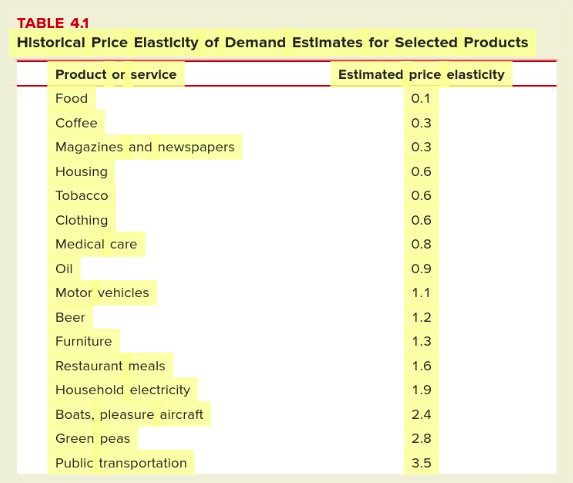
\includegraphics[scale=0.8]{Afsnit/Lektion1/Elastisitet.png}

\subsection{A graphical interpretation of price elasicity}
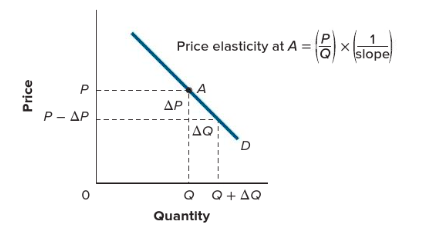
\includegraphics[scale=0.8]{Afsnit/Lektion1/Elastisitetgraf.png}
\begin{align*}
    \text{Priselastisitet} = \in \frac{\frac{\Delta Q}{Q}}{\frac{\Delta P}{P}}
\end{align*}
Hvis man skal bestemme den i et bestemt punkt bruges formlen på grafen. 
\begin{eks} \textbf{} %Nyt eksempel
\newline
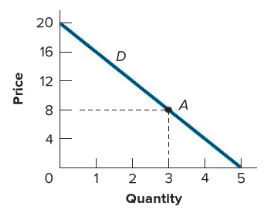
\includegraphics[scale=0.8]{Afsnit/Lektion1/Elastisiteteks.png}

Hvis man skal beregne priselastisiteten i A ser man på forholdet mellem skæring med y og x-aksen.
\begin{align*}
    \frac{1}{\text{slope}} = \frac{1}{\frac{20}{5}}= \frac{1}{4}
\end{align*}
Så ser vi på forholdet mellem mængde og pris i A.
\begin{align*}
    \frac{P}{Q} = \frac{8}{3}
\end{align*}
Dermed har vi
\begin{align*}
    \in_A = \frac{8}{3} \times \frac{1}{4} = \frac{2}{3}
\end{align*}
Det vil sige at når prisen er 8 vil et 3\% fald i pris medfører en stigning på 2\% i mængden
\end{eks}

\subsubsection{Price elasticity changes along a straight-line demand curve}
På midtpunktet af kurven vil priselastistiteten altid være 1. Hvis den er under midtpunktet vil den være under 1 og samme med over. 
\subsubsection{Two special cases}
Det ovenstående gælder selvfølgelig ikke at hvis efterspørgselskurven er vandret er hældningen 0 og derfor er priselastisiteten uendelig ved hvert punkt. Dette kaldes \textbf{perfekt elastisk}. Hvis den er lodret er hældningen uendelig og derfor er priselastisiteten 0 ved hvert punkt. Dette kaldes \textbf{perfekt uelastisk}.

\subsection{Elasticity and total expenditure}
Sælgere er interesseret i at vide hvor meget de kan tage for en vare. Hvis man antager det samlede forbrugere bruger på et produkt er sælgers samlede indtægter. Hvis man har at man kan sælge 500 billetter til 2kr og 400 til 4kr. Vil man vælge at sælge til 4kr da indtjeningen er 1000kr ift 1600kr. Hvis man kun kunne sælge 200 billetter hvis man satte dem til 4kr, ville man vælge de 2kr. 

Ved at beregne på denne måde er det muligt at bestemme den optimale prise for sælger. Dette er ved midtpunktet af efterspørgselskurven. 

\textbf{Regl nr. 1}: Hvis priselastisiteten er over 1, vil prisen og samlede indtægt bevæge sig i hver sin retning. 

\textbf{Regl nr. 2}:  Hvis priselastisiteten er under 1, vil prisen og samlede indtægt bevæge sig i samme retning. 

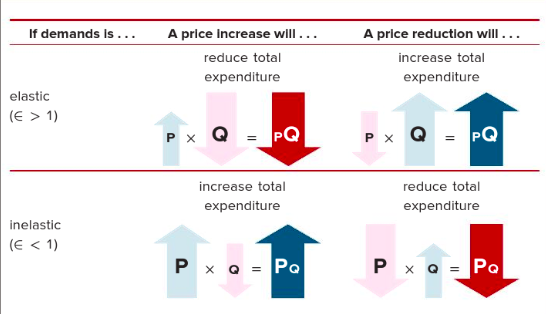
\includegraphics[scale=0.8]{Afsnit/Lektion1/ElastisitetPQ.png}

\subsection{Income elasticity and cross-price elasticity of demand}
\textbf{Krydspriselasticitet af efterspørgsel} er ændring i mængden af en varer ift ændring af pris på en komlementær/erstatning varer. Hvis elasticiteten er negativ er de komplementær vare og hvis den er positiv er de erstatninger. 
\textbf{Indkomstelasticitet af efterspørgsel} er ændring i mængden af en varer ift indkomsten.

\subsection{The price elasticity of supply}
\begin{defn}\textbf{Priselasisiteten for udbud} %Ny definition
\newline
\textbf{Priselasisiteten for udbud} er den procentvise ændring i mængden af udbud ved en prisændring på 1\%
\end{defn}
Den beregnes på samme måde som priselastisiteten for efterspørgsel også i hvert punkt, den er bare altid positiv. Den er altid 1 hvis udbudskurven går gennem origo. Hvis den er lodret er der perfekt uelastisk, vandret perfekt elastisk.

\subsubsection{Determinants of supply elasticity}
Jo nemmere det er at skaffe yderligere input jo højere er priselastisiteten. 
\textbf{Fleksibilitet af inputs}: Hvis et input også kan bruges til et andet produkt kan man tage input derfra og dermed gøre varen relativ elastisk. Det er fx nemt at skaffe folk der kan lave lemonade men svært at skaffe hjerne kiruger. 

\textbf{Mobility of inputs}: Hvis det er nemt at transportere et input, kan man ved en stigning i prisen på et marked gøre det muligt at søge over på et andet marked hvor det måske er billigere. Landbrugsprodukter  er mere elastiske da landmænd er villige til at migrere nord til vækstsæsonen. Priselastisiteten for mange ting stiger hver gang en ny motorvej bliver bygget.

\textbf{Ability to produce substitute inputs}: Hvis der kommer en erstatning vil priselastisiteten stige.

\textbf{Time}: Da det tager tid at skift varer, bygge maskiner mm. Vil elastisiteten være højere på lang sigt end kort sigt.

Flygtige priser er også almindelige i markeder hvor efterspørgselskurverne svinger kraftigt og udbudskurven er meget uelastisk.

\subsubsection{Unique and essential inputs: the ultimate supply bottleneck}
Det er bare ikke altid muligt at få de nødvendige inputs, fx hvis du vil starte et NBA team. De gode spillere er for dyre. På lang sigt er unikke og nødvendige input den sande flaskehals for udbud. 

\subsection{Vigtigt fra forelæsningen}
\textbf{Efterspørgsel}
Efterspørgselskurven laves ud fra reservationspriser. Ved 4kr er der 8000 der vil købe.

Langs kurven, prisen stiger eller falder. 
Kurven flytter sig, prisen på komplementære(ski(pris op), leje til lift(flytter til venstre)) eller substitutter ændres(æble(pris stiger) og appelsinjuice(kurve til højre)). Indkomst stiger, kurve til højre(normal goder). præferencer, befolkningen(fx størrelse) og foventninger(elbil) kan også rykke kurven.

\textbf{Udbud}
Igen er det udbydernes reservationspris der afgør kurven. 

Langs kurven, pris ændres

Kurven flytter, prisen på input ændres(pris på mel stiger, kurve for pizza mod venstre) eller teknologien forbedres(kurve mod højre). Vejret, antal udbydere og forventninger kan også påvirke udbuddet.

\textbf{Ligevægt}
Alle vil gå efter ligevægt.

\textbf{Efterspørgsels priselasticitet}
Hvis kurven skærer y-aksen i a og x-aksen i b, gælder det i ($\frac{b}{2}, \frac{a}{2}$) at $\in = 1$. For på højresiden af $\frac{b}{2}$, $\in<1$ og venstresiden af $\frac{b}{2}$, $\in>1$.

Jo mere stejl en kurve er jo lavere er priselasticiteten. 

\textbf{Monopol}
Når man selv kan vælge en pris vil man aldrig sætte prisen sådan at den er ikke elastisk. Man vil hæve prisen. På samme måde vil man sænke prisen hvis den er elastisk. Man vil gå efter enhedselasticitet da det er den optimale omsætning. 

\textbf{Øvrige elasticiteter}

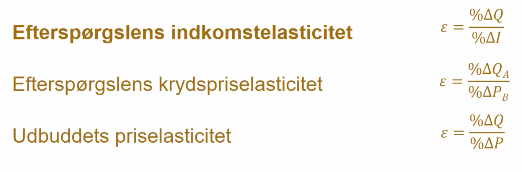
\includegraphics[scale=0.8]{Afsnit/Lektion1/andre.png}




















\chapter{Lektion 2}
\section{Kapitel 5}
\subsection{The law of demand}
\textbf{Loven om efterspørgsel} er det der siger folk gør mindre af det de vil når prisen stiger. 

Man opvejer stadig fordele og ulemper, og man man vil ikke overstige sin reservationspris. Reservationsprisen er der hvor fordele og ulemper går i 0. 

\subsubsection{The origins of demmand}
Reservationsprisen bestemmes blandt andet ud fra ens præferencer. En Justin fan vil give mange penge for et album mens andre ikke ville. Ens præferencer kan stamme fra landet, familien eller skolen du er vokset op i/ved. Det kan også afgøres af andre ting i omgivelserne, fx en populær film om dinosauer vil dinosauerlegetøj stige. Ens forbrug påvirkes også af venner og man gerne vil ses forbruge på det "bedste"(heller flammen i chinabox).

\subsubsection{Needs versus wants}
Ved efterspørgsel kan man skille behov og ønsker ad. Når man fået mad, tag over hoved og det nødvendige tøj så vi er sunde og raske 

\subsection{Translating wants into demand}
Vi har ikke ubegrænsede resourcer og skal derfor fordele dem på de vigtigste ting, og det der giver mest nytte i alt. 

\subsubsection{Measuring wants: the concept of utility}
Nytte er et koncept der repræsentere folks tilfredshed ved deres forbrug. Det at folk prøver at maksimere tilfredsheden, kaldes for nytte maksimering. Hvis at købe en is bringer dig nytte, er det ikke sikkert at købe 10 is vil bringe dig 10 gange så meget lykke, ikke engang hvis de var gratis. 
%

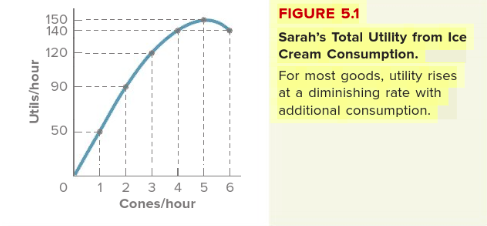
\includegraphics[scale=0.8]{Afsnit/Lektion2/Sarahkoberis.png}

Det ses her at \textbf{marginal nytten} falder fra 50 til 40 til 30 osv, indtil den tilsidst er negativ. Når marginanytten er negativ vil den \textbf{totale nytte falde}. I dette tilfælde vil fordelene overskyde ulemperne til den 5 is, og derfor vil hun købe indtil den 5. Loven om faldende marginalnytte er den lov der beskriver at bare fordi du får dobbelt så meget af noget, bliver du ikke dobbelt så glad. Der er selvfølgelig undtagelser. 

\subsubsection{Allocating a fixed income between two goods}
Det er sjældent man kun skal vurdere nytten for en ting. Hvis man har en bestemt mængde penge der kan bruges på to forskellige produkter skal man vurdere hvordan man får mest mulig lykke ud af det. Ud fra loven om faldende marginalnytte ville det ikke give mening at bruge alle pengene på en af tingene, men fordele dem på de to produkter. Når man vælger den kombination der giver den højeste totale nytte har man opnået \textbf{optimal kombination af varer}. Det kan bestemmes ved at finde der hvor nytten ift penge er det samme for alle varerne, da det her ikke er muligt at hæve den totale nytte. 

\subsection{The rational spending rule}
\begin{defn}\textbf{The Rational Spending Rule} %Ny definition
\newline
Forbrug burde fordeles blandt varerne sådan at marginal nytten per kr. er den samme for hver varer. 
\end{defn}

\begin{itemize}
    \item $MU_C$ - marginal nytte af chokolade i utils per pint
    \item $P_C$ - Pris for chokolade i kr per pint
    \item $\frac{MU_C}{P_C}$ - Marginal nytte per kr i util per kr
    \item Det samme med V for vanilje
\end{itemize}
Så vil man maksimere den totale nytte ved
\begin{align*}
    \frac{MU_C}{P_C} = \frac{MU_V}{P_V}
\end{align*}
Hvis højresiden er større end vestresiden skal man købe mere af højresiden. Det er selvfølgelig ikke alting man kan bruge denne teori på, fx tv. Man må stadig ikke tage gennemsnittet og gå ud fra som ved alt mulig andet i økonomi. 

\subsubsection{Income and substitution effects revisited}
Substitutionseffekten: hvis prisen stiger på en varer skifter man til substitutionen, og dens efterspørgselskurve flyttes til højre. Indkomsteffkten: Hvis indkomsten falder flyttes efterspørgselskurven for normale varer til venstre, folk har ikke råd til lige så meget. 

Hvis prisen på noget stiger vil marginal nytten falde og man vil derfor skulle bruge flere penge på en anden varer istedet for den med prisstigningen, for at opnå maksimal total nytte. 
\subsubsection{Applying the rational spending rule}
Når man ser en stigning i priser og folk skifter til en substitut varer er det fordi at den reel pris stiger. Altså stiger prisen ift andre priser. Det betyder at bare fordi den nominelle pris stiger betyder det ikke at folk skifter, hvis priserne på alt andet også stiger. 

\textbf{The importance of income differences}
Jo flere penge man har jo mere villig er man til at betale mere for ting, da det ikke er en lige så står del af ens indkomst som hvis man ikke tjente meget. 

\subsection{Individual and market demand curves}
Hvis man kender hvert individs efterspørgsel efter en varer, kan man lave en efterspørgselskurve for varen over hele markedet. Det gør man ved \textbf{horisontalt addition}. Hvis der kun er to købere på is-markedet, Sarah og Tom. Sarah efterspørger 2 is til prisen 4kr og Tom efterspørger 3 is til prisen 4kr, så er den samlede efterspørgsel på is-markedet 5 is til prisen 4kr. 

\subsection{Demand and consumer surplus}
\textbf{Forbrugeren overskud} er forskellen mellem prisen og forbrugerens reservationspris. Dette kan bruges til at beregne det totale overskud for alle forbrugere på markedet. 

\subsubsection{Calculating consumer surplus}
\begin{eks} \textbf{} %Nyt eksempel
\newline
Der er 11 købere der hver især kan købe max. 1 vare om dagen. Køber 1 har en reservationspris på 11kr, den næste 10, den næste 9 osv. Efterspørgselskurven vil være en trappe. Hvis den efterspurgtvarer kostede 6kr, ville der blive solgt 6 enheder om dagen. 5 af køberne vil have overskud og den sidste vil gå i 0. Overskudende vil være henholdsvis være 1, 2, 3, 4 og 5 kr. Det samlede overskud ville her være 15kr. 
\end{eks}

Dette kan overføres til en almindelig efterspørgsels og udbudskurve. Bare find arealet af trekanten. På billedet er overskuddet 2000 gallons/day. 

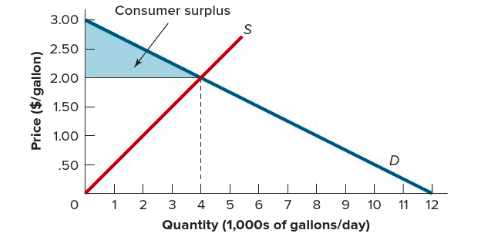
\includegraphics[scale=0.8]{Afsnit/Lektion2/Consumersurplus.png}

\section{Kapitel 6}
Over årene er produktiviteten i mange industrier steget. Industriarbejderes løn er dermed også steget, men en frisør bruger stadig lige lang tid på at klippe en person som for 30 år siden, og lønen for dem er også steget. Dette kan forklares ved at hvis frisøren ikke også fik mere i løn så kunne personen bare vælge et andet jo der gav mere i løn, men problemet er at der stadig er brug for frisører. 

\subsection{Thinking about supply: the importance of opportunity cost}
Udbudskurven laves ud fra offeromkostningerne(alternativomkostninger). Man kan sammenligne det med følgende eksampel.
\begin{eks} \textbf{} %Nyt eksempel
\newline
Harry kan enten tjene 6 kr i timen på hans arbejde eller samle dåser. Nedenfor ses mængden af dåser han kan samle.

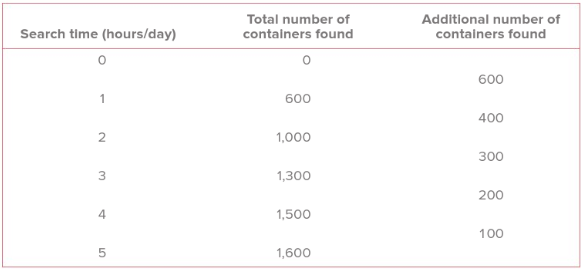
\includegraphics[scale=0.8]{Afsnit/Lektion2/Harry.png} 

Så kan den nødvendige pris for hver dåse bestemmes, for at det kan betale sig at samle dåser.
\begin{align*}
    p(\Delta Q) = 6kr\\
    \text{eks}\\
    p(400) = 6kr \Leftrightarrow p = 1.5 øre
\end{align*}
Ud fra dette kan "udbudskurven" laves.
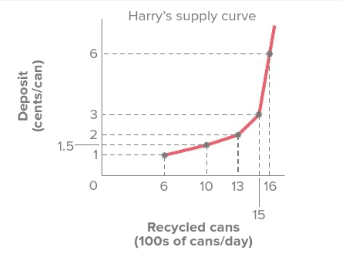
\includegraphics[scale=0.8]{Afsnit/Lektion2/Harry2.png}
\end{eks}

\subsection{Individual and market supply curves}
På samme måde som for efterspørgsel kan man bruge horisontal addition til at gå fra individuel udbud til hele markedets udbudskurve. 

Grunden til kurven har en positiv hælding kan forklares ved \textbf{the principle of increasing opportunity cost} eller \textbf{the low-hanging-fuit principle}. Det er nemmere at finde de første og det bliver dermed sværer og sværer at finde nogle "dåser". Derudover er det på grund af offeromkostningerne, jo højere prisen bliver jo flere dækker det offeromkostningerne for. Ved en lav pris, er der kun få der laver noget hvis offeromkostninger bliver dækket. Hvis vi vender tilbage til eksemplet. En for en arbejdsløs dækker at samle dåser offeromkostningerne for hvad han kunne tjene på et andet arbejde(da han ikke har et). Derimod skal prisen være en del højere før en matematikøkonom får dækket sine offeromkostninger. 

\subsection{Profit-maximizing firms in perfectly competitive markets}
\subsubsection{Profit maximization}
De fleste firmaer eksistere for \textbf{proffittens} skyld, dette er \textbf{profit-maksimerings firmaer}. Et firmas profit er forskellen på det det koster at producere varen for og det forbrugeren giver for den. 

Udbudskurven er lavet ud fra at det er profit-maksimerings firmaer der sælger en vare på et marked med fuldkommen konkurrence(perfekt konkurrence). Hvilket er markeder hvor individuelle firmaer ingen indflydelse på markedsprisen, og derfor er firmaerne \textbf{pristagere}.

\textbf{Fuldkommen konkurrence}:\\
\begin{itemize}
    \item Alle firmaer sælger samme standard produkt. Købere er altså villig til at skifte sælger for at prisen er lavere.
    \item Der er ikke nogen stor købere eller sælgere der kan styre markedet. Det består kun at små = pristagere.
    \item Man kan frit bevæge sig mellem markeder. Der er ingen bindning og alle kan skaffe det de skal bruge for at producere varen.
    \item Sælgere og købere kender alle muligheder. 
\end{itemize}
Hvede er tæt på fuldkommen konkurrence det er computermarkedet ikke, hvor microsoft styre meget, fx priser.

\subsubsection{The demand curve facing a perfectly competitive firm}
Mange af de konklussioner der kommer, kan også passer til udbud/efterspørgsel for  \textbf{ikke-fuldkommen kokurrence firmaer} som fx Microsoft.
Fordi firmaer i fuldkommen konkurrence ikke bestemmer prisen, derfor er deres individuelle udbudskurve en horisontal streg ved markedsligevægt. For hele markedet ser udbud/eftespørgselskurverne "normale" ud. 

\subsubsection{Production in the short run}
Hvordan vurdere man under fuldkommen konkurrence hvor meget man som firma skal producere. \textbf{Faktorerne for produktionen} er de input der er brugt til at producere en varer, fx arbejdskraft eller maskinleje og meget meget mere. \textbf{Kort sigt} er hvor der er nogle ting firmaet ikke kan nå at ændre, fx. de kan ikke bare nå at skifte masiker ud men de kan nå at ændre mængden af arbejdskraft. \textbf{Lang sigt} er hvor alle faktorer kan nå at ændres. 

Når inputs vokser, fx arbejdskraft vil output stiger. Dog vil det ikke stige for evigt. hvis man starter med 1 arbejder og man får 1 til gør de en stor forskel men hvis man har 100, og får 1 til gør det slet ikke det samme. 

\begin{defn}\textbf{Law of diminishing returns} %Ny definition
\newline
Når nogen faktorer i produktionen er holdt fast, vil en stigning i produktionen af en varer på et tidspunkt kræve endnu større stigning i de variable faktorer. 
\end{defn}

\textbf{Faste faktorer} er på kort sigt, dem der ikke kan nå at ændres, og de \textbf{variable faktorer} er på kort sigt dem der godt kan nå at ændres. 

\subsubsection{Some important cost concepts}
En \textbf{fast omkostning} er en omkostning der vil være der ligemeget hvor meget firmaet producere, foreksempel en husleje. Derudover er der \textbf{variable omkostninger} som varierer ift produktionen. De \textbf{totale omkostningerne} er de variable og faste omkostninger tilsammen. 
\textbf{Marginalomkostningerne} er det de totale omkostninger stiger med når man udfører én ekstra aktivitets enhed. Det er definieret som ændringen i de totale omkostning ift ændringen i output. 

\subsubsection{Choosing output to maximize profit}
Hvordan afhænger mængden af produktion af pris, løn og omkostninger af kapital. Det gælder om at maksimere profitten som er indtjening minus omkostningerne. 

\begin{eks} \textbf{} %Nyt eksempel
\newline
Man regner med at man kan sælge alle flasker til markeds prisen 0,35kr 

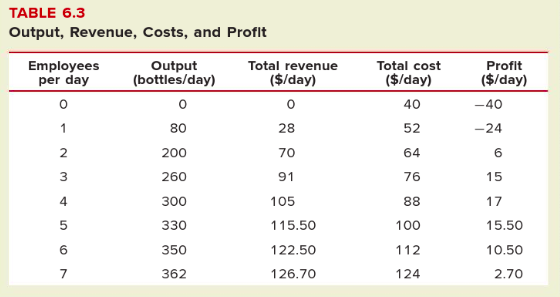
\includegraphics[scale=0.8]{Afsnit/Lektion2/maksprofit.png}

Her ses det at marginalomkostningerne er lavere end marginalfordelene indtil en produktion er på 300 flasker. Det er dermed her man opnår den maksimale profit. Et fald i lønninger vil sænke marginalomkostninger og opnå større profit. På samme måde vil en ændring i faste omkostninger også ændre profitten. 
\end{eks}

\subsubsection{A note on the firms shutdown condition}
Det er ikke altid det kan betale sig for firmaer at producere noget. Hvis prisen er så lav at indtjeningen aldrig overstiger de variable omkostninger, vil de miste mindre ved slet ikke at producere noget. Her vil de så kun have et underskud på de faste omkostninger. Hvis indtjeningen er lavere end de variable omkostninger($\frac{P}{Q}<VC$) kaldes det \textbf{kort sigtet nedluknings tilstand}.

\subsubsection{Averagee variable cost and average total cost}
De \textbf{gennemsnitlige variable omkostninger (AVC)} er de variable omkostninger over antal enheder produceret. Det betyder også at prisen skal være højere end AVC for ikke at komme i kort sigtet nedluknings tilstand(Dividere med Q på begge sider). 

På samme måde kan man bestemme \textbf{gennemsnitlig totale omkostninger} ved at dividere de totale omkostninger med antal enheder produceret. Et firma er \textbf{indbringende} hvis indtjening(PxQ) er højere end de totale omkostninger(ATCxQ)

\subsubsection{A graphical approach to profit maximization}
Det er ikke noget man ikke kan konkludere fra en graf.

\subsubsection{Price=marginal cost: the maximum-profit condition}
Indtil videre har vi kun set på hvis man kan hyre arbejdere i hele tal, hvor profitmaksimering var når marginal omkostningerne var lavere end pricen. Nu ser vi på arbejdere der kan variere kontinuert, og profitmaksimering nu er hvor marginal omkostningerne er lig prisen.

CBP fortæller os at et firma burde producere mere så længe prisen overstiger marginal omkostningerne. Nu hvor arbejdskraften er kontinuert kan man rammer det præcis antal enheder man skal producere for at marginal omkostningerne er lig prisen og det dermed er der hvor man opnår maksimal profit. 

Hvis et firma sælger mere end der hvor marginalomkostningerne og prisen er den samme vil man altid kunne tjene mere ved at sælge og producere færre enheder. Hvis firmaet sælger mindre end der hvor de skærer ville det kunne øge profitten ved at producere mere.

En anden måde end at trække de totale omkostninger fra indtjeningen for at finde profitten er ved at kigge på grafen. 

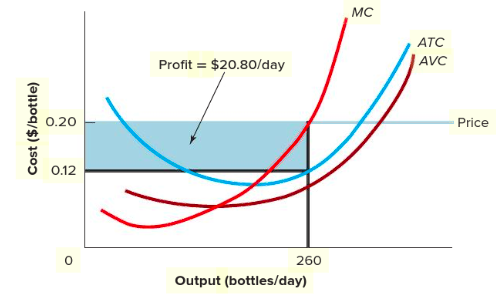
\includegraphics[scale=0.8]{Afsnit/Lektion2/Maksprofit2.png}

Hvis prisen er lavere end de gennemsnitlige total omkostninger vil man have underskud.

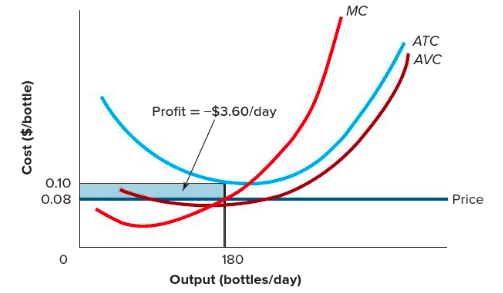
\includegraphics[scale=0.8]{Afsnit/Lektion2/Underskud.png}

\subsubsection{The "law" of supply}
De fuldkommen konkurerende firmaers udbudskurve er kurven for deres marginalomkostninger. For ethvert pris-mængde par langs udbudskurven, er prisen lig sælgerens marginal omkostninger af produktionen. 

\subsection{Determinants of supply revisited}
Hvad kan få udbudskurven til at rykke sig?
\subsubsection{Technology}
Ved teknologisk fremgang bliver det billigere at producere ekstra enheder. Dermed falder marginal omkostningerne og udbudskurven rykkes ned(højre). (sker over tid)
\subsubsection{Input prices}
Ændring i pris af inputs til at producere en varer vil også få udbudskurven til at rykke sig. Hvis lønningerne pludselig stiger, vil marginalomkostningerne stiger og udbudskurven rykker op(venstre). (sker hurtigt)
\subsubsection{The number of suppliers}
Udbudskurven rykker mod højre når antallet af individuelle leverandører vokser. 
\subsubsection{Expectations}
Hvis der er forventninger om at fremtidige priser vil være højere end nutidige priser, holder man på nogle af varerne for at sælge til en højere pris i fremtiden.
\subsubsection{Change in price of other products}
Substitutionseffekten.

\subsubsection{Applying the theory of supply}
Der står ikke noget relevant.

\subsection{Supply and producer surplus}
Som der er noget der hedder forbrugernes overskud, er der også \textbf{sælgers overskud}. Sælgers overskud er forskellen mellem prisen varen sælges for og sælgers mindstepris(reservationspris, marginalomkostning). 

\subsubsection{Calculating producer surplus}
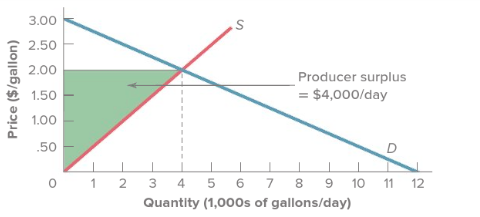
\includegraphics[scale=0.8]{Afsnit/Lektion2/selgeroverskud.png}
Ved ligevægt er overskuddet for sælgerne det stykke der er fra deres mindstepris(kurven) og salgsprisen(trekanten på billedet), og så bare beregn arealet. 


\subsection{Vigtigt fra forelæsningen}

Efterspørgselskurven har negativ hældning pga. loven om aftagende marginalnytte(udover de foregående begrundelser fra lektion 1). Dette gælder da når marginalnytten falder ved at mængden stiger, er folk villige til at betale mindre for det, fordi de får mindre ud af det.

Hvis ens underskud er mindre en ens faste omkostninger skal man bliver ved med at producere da der ville være mere underskud ved ikke at producere end at producere. På lang sigt skal man lukke hvis der er underskud. 

Man vil altid gå efter en produktion der hvor prisen og marginalomkostningerne skærer. Det vil man da det da hvis man sælger mindre udnytter man ikke at man stadig kan sælge mere uden at marginalomkostningerne overstiger ens indtjening per varer. Derudover hvis man er over, vil man for de varer der er over vil man have underskud.

Hvis prisen er under de variable omkostninger er der underskud på kort sigt og de skal lukke. Hvis prisen er under totale omkostninger skal de lukke på lang sigt. 






























\chapter{Lektion 3}
\section{Kapitel 7}
Som verden udvikler sig ændre efterspørgselen sig på forskellige ting, og dermed ændre antallet og diversiteten af sælgere i forskellige markeder sig også hele tiden. Denne ændring sker når det fx bedre kan betale sig at sælge noget andet(offeromkostninger stiger).

\subsection{The central role of economic profit}
\subsubsection{Three types of profit}
\textbf{regnskabsmæssig profit} er indtjening minus eksplicitte(løn) omkostninger. Det er denne profit firmaer bruger i deres årlige rapporter. 

\textbf{Økonomisk profit} er indtjeningen minus de implicitte(offeromkostninger) og eksplicitte omkostninger, hvilket er offeromkostningerne for alle ressourcerne leveret af firmaets ejer. Hvis denne bliver negativ kaldes det et \textbf{økonomisk tab}. Hvis et firma skal blive på markedet på lang sigt skal det økonomiske overskud være over eller lig 0.

Differencen mellem den regnskabsmæssige og økonomiske profit kaldes den \textbf{normale profit}=offeromkostningerne.

\subsection{The invisible hand theory}
\subsubsection{Two functions of price}
Markedsprisen har to roller. Først og fremmest er der \textbf{rationering af pris}. Det sikre at det er de kunder der værtsætter varen mest der får den. Den anden er \textbf{
prisens allokerende funktion}. Det sikre at dirigere ressourcer væk fra overfyldte markeder til markeder der mangler. Disse to er det der blandt andet udgør den usynlige hånd, der rykker rundt på markedet. 

\subsubsection{Responses to profit and losses}
For at et firma skal blive på markedet på lang sigt skal den økonomiske profit være positiv, og dermed tjener mere end den normale profit. I markeder med økonomisk overskud vil der tiltrækkes ekstra ressourcer, og på samme måde vil de forsvinde ved økonomisk underskud.  

\begin{eks} \textbf{} %Nyt eksempel
\newline
Hvis vi siger der er et firma hvis marginalomkostninger er lig markedsprisen når de producere 130.000 bushels, så er det også her hvor der er maksimering af profitten. Det økonomiske overskud beregnes ved at bestemme arealet af nedenstående rektangel. Det er forskellen på de totale omkostninger og prisen. 
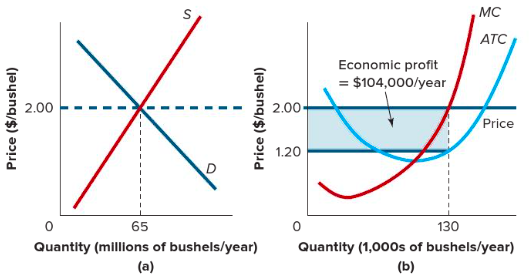
\includegraphics[scale=0.8]{Afsnit/Lektion3/Okonomiskprofit.png}
Her overskrider prisen offeromkostningerne af det det kræver at træde ind på markedet hvis det antages at alt udstyr der kræves er ledig til en konstant pris, og det er gratis at komme ind markedet. 
\end{eks}

I dette eksempel vil der komme flere og flere ind på markedet. Ved at der kommer flere udbydere på markedet vil udbudskurven flyttes mod højre og prisen vil falde. Hvis prisen falder, vil folk blive på markedet og måske endda komme ind på markedet indtil markedsprisen er lig de totale omkostninger. Når dette sker vil den økonomiske profit være lig 0. Det modsatte vil ske hvis prisen er under de totale omkostninger. Det er selvfølgelig ikke alle markeder hvor man bare kan skifte til og fra. Der kan være maskine eller arbejdskraft der ikke er mulig at skaffe og man kan derfor ikke skifte. Dette gør analysen noget mere kompleks. 

Hvis man antager at man bare kan gå ind i eller forlade kornmarkedet på ethvert tidspunkt betyder at kornproduktionen altid kan udvides eller reduceret på lang sigt til en pris på 1kr per bushel. Dette betyder at udbudskurven skal være en horisontal linje lig minimum af de totale omkostninger, 1kr per bushel. 

Ved prisen der er lig minimum af de totale omkostninger, vil hver udbyder have en økonomisk profit på 0. Dette er den langsigtede ligevægt. Det er også her til den bestemte pris at udbyderen oplever den maksimale profit og det er her køberne skal give det det koster at producere varen. 

\begin{eks} \textbf{} %Nyt eksempel
\newline
Hvis der for frisører og massører gælder at der er et økonomisk overskud på 0. Hvis der sker noget der sker noget så efterspørgselskurven for frisører forskydes til venstre og for massører forskydes til højre, vil der komme et nyt kortsigtet ligevægtspunkt for dem og prisen ændres. 

Da de begge startede med et økonomisk overskud på 0, vil frisøren opleve underskud og massøren overskud nu. Derfor vi frisører forlade faget og der vil komme flere massører til, dermed vil udbudskurverne flyttes mod venstre(frisør) og højre(massør). Dette vil ske indtil den langsigtede ligevægt nås. Det vil være den samme pris som der var ved udgangspunktet, men der vil være færre frisører og flere massører. 
\end{eks}

\subsubsection{The importance of free entry}
Hvis det ikke er muligt at træde ind i et marked hvor der er et økonomisk overskud vil markedet ikke gå mod langsigtede ligevægt. Dette kan skyldes \textbf{hindringer i at indgang}, fx copyright, lovmæssige krav og praktiske ting. På samme måde kan der være \textbf{hindringer i at forlade markedet}.

\subsection{Economic rent versus economic profit}
\textbf{Økonomisk leje} er forskellen mellem udbyderens reservationspris og salgsprisen. 

\begin{eks} \textbf{} %Nyt eksempel
\newline
Hvis der er 100 resturanter hvor af 99 af dem betaler deres kokke 30.000kr om året hvilket er det samme som de ville kunne tjene ved at lave noget andet. Den sidste koks mad er så godt at folk vil betale 50 procent mere for det end andre steder. Ejerne af de 99 resturanter tjener hver 300.000kr hvert år som er præcis det samme som deres normale profit. Da kunderne ved den sidste resturant er villige til at betale 50 procent mere, tjener resturanten 450.000kr om året. På lang sigt skal konkurrence sikre at kokken får 180.000kr om året. 30.000kr som de nomale kokke får og 150.000 ekstra fra den ekstra indtjening. Kokkens reservationspris er 30.000kr om året da det er det hun kan tjene i et andet fag og derfor er hendes økonomiske leje 150.000kr om året. Den økonomiske profit for ejerne af resturanten er 0. Resturanten ejer er nødt til at betal kokken de 180.000kr for eller er der andre der ville byde på kokken og det ville ske indtil der var nogen der bød 180.000. Efter dette ville det ikke kunne betale sig.
\end{eks}

\subsubsection{The invisible hand in action}
\textbf{How do cost-saving innovation affect economic profit in the short and long run?}:\\
Hvis der sker en forbedring som den økonomiske profit stiger vil der ske følgende. Hvis det kun er indenfor et enkelt lille firma denne forbedring sker, vil der ikke ske noget med markedsprisen og firmaet vil tjene mere. Når flere og flere firmaer får forbedringen vil udbudskurven forskydes nedad da marginal omkostningerne falder, og markedsprisen vil hermed falde. Derfor falder den økonomiske profit igen til det oprindelige. Den langsigtede udbudskurve vil tilsidst være forskudt ned og alle vil tjene deres normal profit. Hvis der er firmaer til denne tid der ikke har fået forbedringen endnu vil de få et økonomisk underskud. 

\subsection{The distinction between an equilibrium and a social optimum}
Når ligevægt er nået er der ikke mulighed for at optimere mere for individer. Det betyder ikke at det ikke er muligt at være bedre stillet når markedet ikke er i ligevægt. Nogle gange kan firmaer tjene meget ved at være de første til at gøre noget, fx købe en nye slags maskine. Det er formentlig nogen der virkelig har styr på markedet eller er heldig. 

\subsubsection{Smart for one, dumb for all}
Overskriften siger ligesom det hele....

\subsubsection{Market equilibrium and efficiency}
Når økonomer taler om \textbf{effektivitet} eller \textbf{Pareto effektivitet} har det en meget snæver teknisk mening. Når man siger at markedsligevægt er effektivt menes følgende: \textit{Hvis prisen og mængden er andet end ved ligevægtværdierne, vil man altid skade andre ved at hjælpe nogen}. Det er dermed effektivt ved at i ligevægt kan man hjælpe nogen uden at skade andre. Køber eller sælger er frustreret. Hvis prisen er over ligevægt vil det gavne alle hvis prisen faldt, da det vil komme tættere på alles reservationspris, derfor kan det ikke være effektivt at sælge over ligevægt. På samme måde kan det også kun blive bedre for begge parter hvis prisen stiger. Dermed kan det konkluderes at det i det frie marked gælder at det er mest effektivt i ligevægt. 

Dette holder dog kun hvis der er fuldkommen konkurrence, og opfylder andre restriktioner. Fx hvis udbudskurven ikke inkluderer alle omkostninger. Hvis en udvidelse af output resulterer i mere forurening vil koste mere end indikeret på markeds udbudskurven. Dermed vil ligevægt output være høj ineffektiv og ligevægts prisen være lav ineffektiv. Det kan også være at kurverne ikke får alle fordele med mm.

\textbf{Efficiency is not the only goal}: Ligevægt resultere i maksimal økonomisk overskud. Effektiv $\neq$ godt. Noget så simpelt som indkomst, kommer ind i spillet her. Når markedet for mælk er effektivt ved en pris på 8,50kr per liter, er det ikke alle der har råd til det. Sådan vil det være på mange markeder, at bare fordi det er effektivt er det ikke godt for alle. Nogle gange skal man lave regler for visse marked så man er sikker på at alle har en mulighed for at få noget. 

\textbf{Why efficiency should be the first goal}
Effektivitet er et mål da det hjælper os med at nå vores andre mål bedste/mest muligt. Ved ligevægt er det altid muligt at generere yderligere overskud.

\subsection{The cost of preventing price adjustments}
\subsubsection{Price ceilings}
Fx da priserne steg helt vildt i 70'erne pga stoppet af olielevering fra mellemøsten, lavede man i USA et loft på hvor meget olien måtte koste for at sikre at fattige familier ikke frøs ihjel i deres hus. Dette gør dog at der tit sker et fald i økonomisk overskud for udbyderne. Nedfor ses der 2 figurer den første viser uden et prisloft og den anden viser et prisloft på 1dollar/gallon. Beregn de blå og grønne arealer for at finde overskud for køber og udbyder.

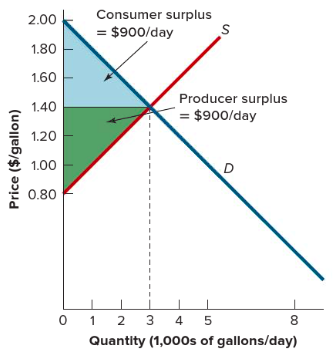
\includegraphics[scale=0.5]{Afsnit/Lektion3/loft1.png}

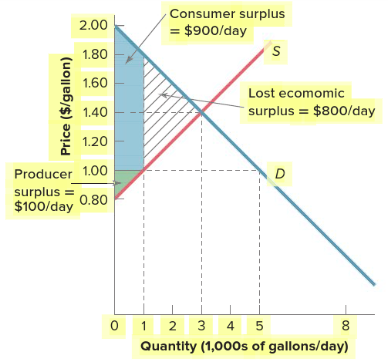
\includegraphics[scale=0.5]{Afsnit/Lektion3/loft2.png}

Ved lavere pris vil dem med mindre reservationspris købe mere end dem med højere reservationspris. Det vil ske da dem med højere reservationspris vil stadigvæk have et overskud hvis prisen bare stiger en smule. Derudover kan en reduktion i pris også gøre at folk vil gøre mere for at få fat i varen, fx stå i lange køer og stå tidligt op. 

Men hvorfor giver man ikke bare de fattige nogle flere penge istedet for at sætte et prisloft, som giver et større tab i total overskud. Udbydere vil nok være mere villig til at betale en smule mere i skat hvis de slipper for et stort tab. Disse skatter kunne bruges på at hæve indkomsten for de fattige som ville få stor gavn af det. Begge ville få mere gavn af dette og det er derfor man burde gøre det istedet for at indføre et prisloft. 
Det kan dog betyde at for fattige er det mindre attraktivt at arbejde, men det kommer i et andet kapitel.

\subsubsection{Price subsidies}
Regeringen kan sælge til en lavere pris end verdensprisen. Når de gør det kan der stadig ske et fald i det totale økonomiske overskud. Det sker da det er skattepenge der alligevel skal betale den "rabat" regeringen giver. Eks på side 196-197.

Alt i alt. Problemet er at fattige familier tjener for lidt. Den simpleste og bedste løsning bare at give dem flere penge. 

\subsubsection{Vigtigt fra forelæsningen}
Som revisor ser man på profit som egentlig profit(regenskabsmæssig profit). Økonomer ser også på offeromkostningerne(økonomisk profit). Offeromkostningerne kaldes normal profitten. 







\chapter{Lektion 4}

\section{Kapitel 8}

Hvis man vil undgå at ens produkt går mod ligevægt og man ikke længere får et stor overskud skal man have \textbf{copyright}. Dette bliver så til et ikke fuldkomment konkurrerende marked, eller et prissætte marked. 

\subsection{Perfect and imperfect competition}
Økonomer adskiller for det meste mellem tre forskellige typer af ikke fuldkomne markeder. 

\subsubsection{Different forms of imperfect competition}

Længst fra fuldkommen konkurrence er rent monopol. Hvilket er hvor der kun er en sælger på markedet. 

\textbf{Monopolistic competition}: Det er et marked hvor mange rivaler sælger et produkt der er tæt på hinanden, men ikke helt perfekte substitutter. Der er altid en eller anden ting ved hvert produkt der gør at nogle kunder ville foretrække varen. Det har en ting til fælles med fuldkommen konkurrence, hvilket er at man kan komme og gå fra markedet som man vil. Et eksempel på monopolistisk konkurrence er lokale olieselskaber, her er produktet egentlig det samme men placeringen for tanken spiller en stor rolle for forbrugeren. Hvis kunderne foretrækker en vare frem for en anden kan producenten hæve prisen en smule uden at miste nogen kunder. Dette betyder dog ikke at firmaet vil opleve økonomisk profit på lang sigt. Hvis andre firmaer kunne se at der var profit i markedet ville de komme ind på det, og selv om de ikke ville kunne producere det præcis samme vare ville prisen stadig presses ned. Dette vil ske da andre måske ser større fordele i det nye produkt og derfor vil de gamle miste kunder. Altså vil firmaerne i markedet igen ende med en økonomisk profit på 0.

Indenfor denne markedstype skal producenterne ikke bare vælge prisen med omhu men også varen. Hvor meget skal den afspejle en anden vare?

\textbf{Oligopoly}: Mellem fuldkommen konkurrence og monopol ligger oligopol, hvilket består af få store firmaer. Ligesom monopol er oligopol tit en konsekvens af omkostningsfordele, der forhindre mindre firmaer i effektivt at konkurrere. Under oligopol sælger producenterne tit det samme produkt, fx cement. Firmaer der er på et marked der er under oligopol, skal fokusere på prissætningen og reklamen frem for produktet. Omkostningsfordele tilknyttet store størrelser er for det meste vigtigt under oligopol, og det vil helt klart gøre at adgang og at forlade markedet vil gøre at den økonomisk profit er 0. Det er ikke sikkert at selvom at to firmaer på et oligopol marked har et økonomisk overskud at hvis en tredje træder ind i markedet at det også vil have overskud, eller måske alle tre nu vil have underskud på grund af en lavere pris. 

Fra nu af vil en fra et af de tre ikke fuldkomne markeder kaldes en monopolist i dette kapitel.

\subsubsection{The essential difference between perfectly and imperfectly competitive firms}

\textit{Firmaer i fuldkommen konkurrence står med en perfekt elastisk efterspørgselskurve for deres produkt, hvorimod firmaer i ikke fuldkommen konkurrence står med en efterspørgselskurve med en negativ hældning.} Der er en ligevægtpris på det fuldkomne marked der ikke giver nogen mening at afvige fra da det er der de sælger alle deres varer. Derfor er efterspørgselskurven en horisontal linje. Hvis et firma i ikke fuldkommen konkurrence derimod sætter prisen lidt op, er det ikke sikkert at det er alle der forlader "ham", og derfor har efterspørgselskurven en negtiv hældning. 

\subsection{Five sources of market power}
De firmaer der har en efterspørgselskurve med negativ hældning siges at nyde markeds krafterne, som referer til deres mulighed om at ændre priserne. Eksklusiv kontrol over inputs, patent og copyright, offentlige licenser, stordriftsfordele og netværksøkonomier er 5 ting der gør at konkurrencen bliver begrænset og det dermed er muligt at nyde markeds krafterne. 

\subsubsection{Exclusive control over important inputs}
Hvis et firma kontrollere et essentielt input til en vare har det firma markeds kraften. Fx mange vil betale meget for et kontor i USAs højeste bygning. Ejeren af WTC har markeds kraften.

\subsubsection{Patents and copyright}
Hvis man har patents eller copyright på noget er man den eneste der må tjene på det og derfor udelukker det andre fra at producere varen. Fx. medikamenter. 
\subsubsection{Government licenses or franchises}
Temmelig meget argumentet ovenfor.

\subsubsection{Economies of scale and natural monopolies}
Hvad sker der når et firma fordobler alle faktorerne i produktionen? Hvis output fordobles, siges produktions processen at være konstant vender tilbage til skala. Hvis output mere end fordobles sige produktions processen at have stigende vender tilbage til skala. I begge tilfælde vil den gennemsnitlige omkostning falde når produktionen stiger. Et monopol som resultat af stordriftsfordele kaldes naturlig monopol.

\subsubsection{Network economies}
Populariteten af en vare kan også afhænge af hvor mange der har varen. Hvis der er to forskellige varer, men der er en af dem der har noget der er en smule mere attraktiv, køber folk den. Selv hvis vare to formår at få den samme ting, vil folk allerede have valgt en ting, og dermed er der bedre muligheder for at tilgå denne vare, få den repereret mm. Der er fx Microsoft, selvom der måske er et brand der kan det samme, er det nemmere af få det andet og man har formentlig allerede andet der kan arbejde sammen med brandet. Det er dog ikke altid at man bare kan antage at fx. Microsoft forbliver ene på markedet, det har man kunne se de seneste år mht Apple. Netværksøkonomier, er en naturlig kilde til monopol. 

\subsection{Economies of scale and the importance of start-up costs}
Variable omkostninger af output, det gør faste omkostninger ikke, og der er ingen faste omkostninger på langt sigt da alle input kan varieres. Dog er der nogle ting hvor opstarts omkostningerne koster meget, og har en meget lav marginal omkostning. Dette kan fx være et software firma, hvor det kræver meget i starten at skrive koden, men når det er færdigt er resten billigt at "producere". Disse firmaer er underlagt betydelige stordriftsfordele, da de gennemsnitlige totale omkostninger vil falde når produktionen stiger, ATC = (fasteomkostninger / antal producerede) + marginal omkostningerne.

\begin{eks} \textbf{} %Nyt eksempel
\newline
Nintendo og Sony har begge faste omkostninger på 10.000.000 og en marginalomkostning på 0.20 per spil. Nintendo producerer 1 mio units og Sony producere 1.2 mio units.  

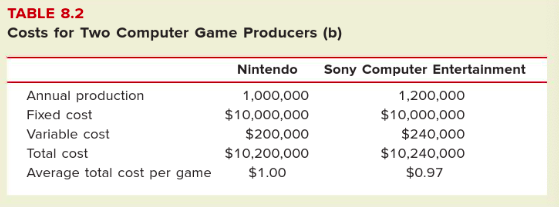
\includegraphics[scale=0.8]{Afsnit/Lektion4/Nintendoogsony.png}

Det ses her at Sony vil have mulighed for at sætte prisen lavere end Nintendo, og hvis man antager at der ikke er andet end prisen der adskiller de to, vil det gøre Sony noget mere populær end Nintendo. For at Nintendo kan sætte prisen ned skal de producere mere, så deres gennemsnitlige totale omkostninger falder. 
\end{eks}

\subsection{Profit maximization for the monopolist}
Så længe fordele overskrider omkostningerne vil firmaer producere mere, altså de marginale fordele der stiger for hver producerede vare kaldes \textbf{marginale indtægter.} De marginale indtægter for at firma i fuldkommen konkurrence er lig markedsprisen 

\subsubsection{Marginal revenue for the monopolist}
\textit{For en monopolist, er de marginale fordele ved at sælge en ekstra unit lavere end markedsprisen. } Forskellen for firmaer under fuldkommen konkurrence og monopolister, er at underfuldkommen konkurrence kan firmaer sælge alle de units de vil til markedsprisen hvor monopolisterne skal sætte prisen ned for at sælge mere.

\includegraphics[scale=0.8]{Afsnit/Lektion4/marginalindtægt.png}

På grafen se at ved at sælge 2 units, vil firmaet tjene $2 \codt 6 = 12$ og ved 3 units, vil de tjene $3 \cdot 5 = 15$. Altså er de marginale indtægter $3$. I ovenstående eksempel ses det også at den marginale indtægt vil være faldende og når den er lig nul. Hvis efterspørgselskurven skærer andenaksen i a, vil marginal indtægten være nul ved $\frac{a}{2}$ eller hvis den skærer med førsteaksen i b vil marginal indtægten være nul ved $\frac{b}{2}$. Altså hvis eftspørgselskurven kan beskrives ved $D = a - qb$ så er kurven for marginalindtægten $MR = a - 2qb$. 

\subsubsection{The monopolist's profit-maximizing decision rule}
\textit{Profitten er maksimeret på det niveau af output hvor marginal indtægten er præcis lig marginal omkostningerne}. Ved denne definition kan vi se at fuldkommen konkurrence er et specialtilfælde af monopol reglen. Når firmaer i fuldkommen konkurrence udvider med en unit, vil marginal indtægten være lig markedsprisen, fordi de kan udvide salget ved at sænke prisen af de eksisterende units. Så når firmaer i fuldkommen konkurrence sidestiller prisen med marginal omkostningerne, sidesætter de også marginal indtægten med marginal omkostningerne. \textit{Den eneste signifikante forskel mellem de to sager vedrører således beregning af marginale indtægter}

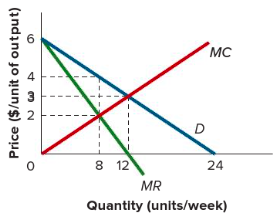
\includegraphics[scale=0.8]{Afsnit/Lektion4/maksimeringafprofit.png} \label{marginalindtægt}

Ovenstående graf viser marginal omkostningerne, efterspørgslen og marginal indtægten. Her ses det at profitten maksimeres når der sælges 8 units om ugen. 

\subsubsection{Being a monopolist doesn't guarantee an economic profit}
Selvom profit maksimerings prisen altid er over marginal omkostningerne, betyder ikke nødvendigvis ikke at der er økonomisk profit. Det sker hvis de gennemsnitlige totale omkostninger er højere end prisen hvor marginal indtægterne er lig marginal omkostningerne. Hvis de gennemsnitlige totale omkostninger er lavere en prisen hvor marginal indtægterne er lig marginal omkostningerne er der økonomisk profit. Nedenstående grafer viser et firma med henholdsvis økonomisk tab og profit. 

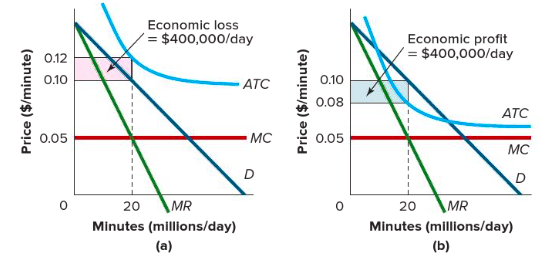
\includegraphics[scale=0.6]{Afsnit/Lektion4/tabogprofit.png}

\subsection{Why the invisible hand breaks down under monopoly}
Er maksimering af profitten det mest effektive for samfundet? Hvis vi ser på grafen i \autoref{marginalindtægt}, ved profitmaksimering ved 2 units vil en stigning med en unit gøre at marginal fordelen stiger med 4 og på det tidspunkt er marginal omkostningerne kun 2, 4-2=2, altså vil samfundet have godt af en stigning med en unit. Da dette ikke gøre er markedet ineffektivt. Monopolististen hæver ikke produktionen da det ikke altid er muligt at holde prisen på de eksisterende units, og kun sænke prisen for den ekstra unit. 

For at opnå social effektivitet, skal monopolisten hæve produktionen indtil marginal fordelene til samfundet er lig marginal omkostningerne, hvilket på figuren er 12 units, altså der hvor efterspørgsel og marginalomkostningerne skærer. 

Det at marginal indtægten er under prisen for monopolisten resultere i \textbf{dødvægts tab}. Det beregnes ved arealet af trekanten under. 

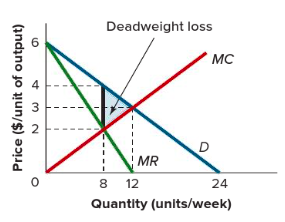
\includegraphics[scale=0.7]{Afsnit/Lektion4/trekantensareal.png}

Da fuldkommen konkurrence er effektivt, men monopol ikke er burde ting som patent så være ulovligt. Nej, det ville dræbe innovation, hvilket også styrker et samfund mm. 

\subsection{Using discount to expand the market}
Da monopoly er ineffektiv betyder det at man kunne gøre noget bedre for nogen uden at skade andre, alle kan få et større stykke af kagen. Hvorfor sælge en monopolist ikke bare itl en pris til nogen og når dem der vil give den pris har købt sætter han prisen ned?

\subsubsection{Price discrimmination defined}
Det gør nogen! Nogen betaler en pris andre en anden, dette er \textbf{prisdiskrimination}, fx seniorrabat. Nogen markeder virker det, andre gør det ikke. 

\subsubsection{How price discrimination affect output}
Hvordan påvirker prisdiskrimination monopolistens profit maksimering? 

\textbf{Perfekt diskriminerende monopolist} betyder at monopolisten tager præcis køberens reservationspris for en vare. Ved at gøre dette vil det totale økonomiske overskud være maksimeret ift hvis man ikke prismaksimerer. Dog vil kunder ikke være særlig glade for at handle med et sådan firma, da deres økonomiske overskud altid vil være 0. Perfekt diskrimination, vil heller aldrig ske da ingen sælger kender alle købernes reservationspriser. Dog er ikke perfekt pris diskrimination muligt. 

\subsubsection{The hurdle method of price discrimination}
For at maksimere profitten vil alle sælgere altid gå efter at sælge til højeste pris en køber vil give. To ting forhindre sælgeren i at gøre dette. Først er der det at sælgeren aldrig helt ved hvad køberen vil give og andet er at de har brug for nogle midler til at forhindre købere med høj reservationspris i at købe til en lav pris. \textbf{Hindringsmetoden til pris diskrimination} løser begge disse problemer ved at køberen skal overvinde en hindring for at være berettiget til rabat. Fx. man skal sende en rabatkupon på mail for at få rabat. \textbf{En perfekt hindring} er når købere præcis bliver inddelt i grupper med deres reservationspris, men det eksistere ikke rigtig. 

\subsubsection{Is price discrimination a bad thing?}
Både sælgers og det totale forbruger overskud vil være det samme eller højere hvis der er pris diskrimination. Dette sker da man ved prisdiskrimination tit oplever at dem der normalt ikke vil købe, køber under pris diskrimination, og da deres reservationspris ikke altid er det samme vil der være nogen kunder der oplever et overskud. Hvis man ligger dette overskud oveni det der tjenes fra dem der altid betale fuld pris, stiger det totale overskud(se eks fra s. 223-225. Da begge parter oplever en fremgang gør pris diskriminationen mere effektiv end bare at kræve én pris fra alle. 

\subsubsection{Examples of price discrimination}
Hindringer er fx black friday, eller bare andre perodiske rabatter, hvor hindringen her er at finde tiden og stedet hvor rabatten finder sted, og prioritere at tage tid til at tage derhen. Andre eksempler er antallet af tilbehør i en ny bil, om en bog er i hard cover eller bare en papirudgave eller om man flyver buisness eller economy. 

\subsection{Public policy toward natural monopoly}
Ved monopol bliver markedet meget mindre effektivt, og da sælgeren oplever et økonomisk overskud på bekostning af forbrugerne. Mange forbrugere har det derfor heller ikke helt godt med at købe fra en monopolist. Regeringer prøver steder at kontrollere monopolisterne på den ene eller anden måde. nogle tager styringen over monopolet og andre prøver at lave love for at kontrollere priserne, men disse politikker skaber økonomiske problemer i dem selv. Så det gælder om at komme op med en måde at skabe størst muligt overskud af fordele over ulemper. 

\subsubsection{State ownership and management}
Monopol er ineffektiv da maksimerings prisen altid er større end marginalomkostningerne. Da monopol er defineret som stordriftsøkonomier, hvor marginalomkostningerne altid er under de gennemsnitlige totale omkostninger, vil det at sætte prisen lig marginalomkostningerne ikke kunne dække de totale omkostninger. Dette resulterer i et tab. En måde at forbedre effektiviteten på er at regeringen tager over industrien, sætter prisen lig marginalomkostningerne og tager skattepenge til at finansiere tabet. Problemet ved dette er at hvis en privat monopolist skærer i omkostningerne med 1kr, stiger profitten med 1kr. Hvis en offentlig monopolist skærer i omkostningerne med 1kr, skærer de i budgettet for monopoliet med 1kr. 
\subsubsection{State regulation of private monopolies}
Hvis regeringen ikke køber hele markedet kan de anvende cost-plus reguleringer. Dette betyder at regeringen går ind sætter prisen for hver monopol så det dækker omkostningerne plus en mark-up så de er sikre en normal tilbagevenden af deres investeringer. 

\textbf{Pitfalls:}
\begin{itemize}
    \item Det er svært at bestemme hvilke af firmaets udgifter der skal inkluderes i det prisen skal dække. 
    \item Firmaer har ingen grund til at finde på ting der kan sænke omkostningerne da de er sikre på at få dem tilbage. Måske vil de endda hæve omkostningerne pga. markuppen. 
    \item Det løser ikke problemet om at vi gerne vil sætte prisen lige marginal omkostningerne. 
\end{itemize}

\subsubsection{Exclusive contracting for natural monopoly}
En af de bedste metode er at regeringen inviterer private firmaer til at byde på monopol markedet. Regeringen siger hvilket marked det handler om og hvor meget de vil betale for en service, så vinder den lavest bydende. Her vil firmaer stadig være interesseret i at mindske omkostningerne, byde-rundten gør at det er så fair som muligt mht til profitten og hvis regeringen giver penge til de vindende kan prisen sættes til marginal omkostningerne. Denne mulighed er kun mulig ved simple ting som fx skraldemænd og brandmænd, ellers kan det kræve meget komplekse investeringer i kapital.

\subsubsection{Vigorous enforcement of antitrust laws}
I 1890 blev det gjort ulovligt at lave en sammensværgelse om at "lave monopol eller forsøge at lave monopol", som fx Rockefellers. I 1914, ville de forebygge at firmaer arbejdede samme om at danne monopol. Disse \textbf{antitrustlove}, hjælper med at forhindre karteller eller firmaer i at hæve prisen. De fremmer også konkurrencen, men gør også at det ikke er muligt at blive en stordriftsøkonomi. 

\textbf{Til sidst er der den mulighed at man bare kan lade monopolet være et monopol.} For det meste sættes prisen ikke fuldstændig åndssvagt højt, og meget af den profit monopolet tjener skal alligevel betales tilbage i firma skat mm. 











\chapter{Lektion 5}

\section{Kapitel 9}
Udbetalling afhænger af mange ting, handling, tid mm. Her vil der ses på hvordan få principper i spilteori kan hjælpe os med at forstå handlingen fra oligopolister og monopolistisk konkurrenter. 

\subsection{Using game theory to analyse strategic decisions}
I ethvert spil afhænger dit træk af hvordan din modstander reagere på det, og derfor går det ud på at kende din modstanders næste træk. 

\subsubsection{The three elements of a game}
Det er tre \textbf{basis elementer} i et spil: spillerne, mulige "træk og strategier" og de udbetallinger spillerne kan få ved et træk. 

\begin{eks} \textbf{} %Nyt eksempel
\newline
Antag at United Airline og American Airlines var de eneste på Chicago-St Louis ruten. Hver har en økonomisk profit på 6.000kr per flyafgang. Hvis en af dem hæver reklame omkostningerne med 1000kr, vil deres profit stige til 8.000kr mens modstanderens profit vil falde til 2.000 kr. Hvis begge hæver reklameomkostningerne med 1.000kr vil begges profit falde til 5.500kr. 

\textbf{Basiselementerne:} De to flyselskaber, strategierne er at bruge mere eller ikke bruge mere på reklameomkostningerne, udbetalingerne er de fire forskellige mulige udfald ud fra valget om reklameomkostningerne. Disse kan ses på \textbf{udbetalings matricen} nedenfor.

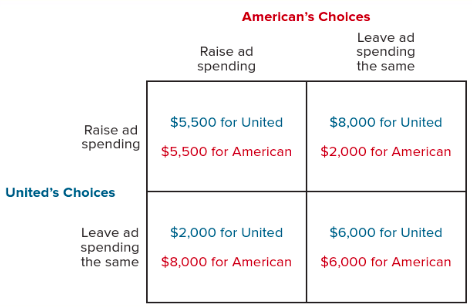
\includegraphics[scale=0.4]{Afsnit/Lektion5/udbetalingsmatrice.png}

\textbf{Dominant strategi} er en strategi der giver en højere udbetaling lige meget hvad andre spillere vælger. Alle andre strategier end denne er de \textbf{dominerede strategier}. I dette tilfælde vil man formentlig vælge ikke at bruge mere, da man vil forvente at hvis en hæver reklameomkostningerne vil den anden også hæve reklameomkostningerne da de ikke er interesseret i en mindre profit. Her vil begge parter tjene mindre end hvis de bare lader reklameomkostningerne forblive på det samme niveau. \end{eks}

\subsubsection{Nash Equilibrium}
Et spil siges at være i ligevægt hvis alle spilleres strategier er det bedste de kan vælge givet andre spilleres valg. Dette kaldes \textbf{Nash ligevægt}. Når dette er opnået er der ingen af spillerne der ville få noget ud af at ændre strategi. Hvis der er en dominant strategi, vil ligevægten være der hvis begge parter følger denne. Man kan stadig nå ligevægt selvom der ikke findes en dominant strategi, det vigtige er bare at hvis man er i ligevægt, vil man tabe noget nogen anden vælger en anden strategi. 

\subsection{The prisoner's dilemma}
\textbf{Fangens dilemma} er når alle spillere vælger den dominante strategi og dette resulterer i en lavere udbetaling end hvis man valgte en domineret strategi. 

\subsubsection{The original prisoner's dilemma}
Se side 242-243, det giver mening. De snakker bare om to fanger der har samme problem som de to flyselskaber. 

\subsubsection{The economics of cartels}
\textbf{Et kartel} er ethvert koalition/forening af firmaer der begrænser produktionen for at få højere økonomisk profit. Kartel dannelse er et klassisk eksempel på hvordan fangernes dilemma kan opstå.

\begin{eks} \textbf{} %Nyt eksempel
\newline
To firmaer sælger vand og vælger at forme et kartel så de kun producere halvdelen af deres normale produktion og sælger til monopolpriser. Da aftalen ikke er lovligt lavet er der ikke noget der stopper den ene producent fra at sælge til en lavere pris, og dermed få hele markedet. Producenternes udbetalings matrice ses nedenunder.

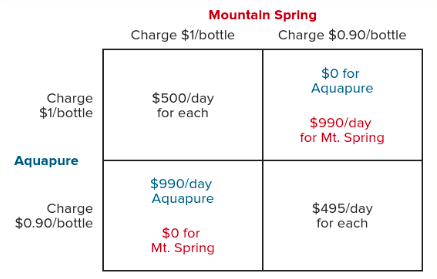
\includegraphics[scale=0.7]{Afsnit/Lektion5/udbetalingsmatriceforvand.png}

Hvert firma ved at ved at sætte prisen en smule ned kan de vinde hele markedet tilbage og få en temmelig højere økonomisk profit. Her vil det andet firma svarer igen og den samlede profit for dem begge vil falde. Dette kan forsætte til de når marginalomkostningerne. Derfor er karteldannelse historisk kendt for at være ustabile. 
\end{eks}

\subsubsection{Tit-for-tat and the repeated prisoner's dilemma}
Når der er nogen firmaer der er i fangernes dilemma flere gange med hinanden kan man lede efter måde at "straffe" et firma hvis de afviger. Når firmaer er i fangernes dilemma med hinanden flere gange, kaldes det for \textbf{gentagne fangernes dilemma.} Der er en strategi der har bevist sig meget nyttig i disse situationer, det kaldes for \textbf{tit-for-tat}. Det går ud på at man gør det "modstanderen" gjorde sidste gang. Dette gør at firmaer ikke afviger da dette vil blive straffet med "hævn" næste gang. Dette virker dog kun når der er to firmaer. 

Nogle gange kommer profitten også an på tidspunktet man udvikler eller laver sit træk. Dette kan beskrives ved et \textbf{beslutnings træ} eller \textbf{spil træ}. Dette ses nedenunder, hvor det er to bilforhandlere der skal beslutte om de skal udvikle en hybrid model. 

\includegraphics[scale=0.5]{Afsnit/Lektion5/spiltræ.png}

Her har Dodge førstevalg, og skal self vælge at lave en hybrid da Chevrolet så vælger ikke at lave en fordi det vil give størst mulig profit. 

\subsubsection{Credible threats and promises}
En \textbf{troværdig trussel} er en hvor den der truer's interesse er at føre truslen ud i livet når tiden kommer. På samme måde er der også \textbf{troværdige løfter}.

\subsubsection{Monopolistic competition when location matters}
Selvom det tit er tilfældet at den der har det første træk har en fordel, gælder dette ikke altid. 

\begin{eks} %Nyt eksempel
\newline
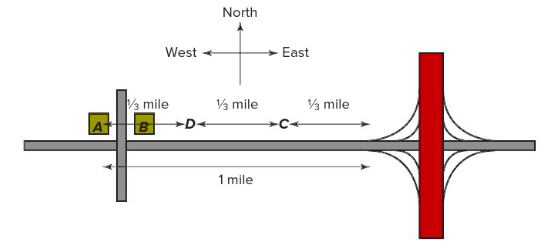
\includegraphics[scale=0.6]{Afsnit/Lektion5/motorvej.png}

Her ses det at A først vælger at have en butik og derefter er der en ny der åbner en butik B. Kunderne tager den butik der er tættest på dem og derfor vil B nu få alle kunderne hen til motorvejen(rød) istedet for A. Derudover vil B aldrig ligge sig ved punktet C da mellem C og A ville kun den halvdel af kunder der lå tættest på C handle der, resten ville gå i A. Det er også derfor at butikker tit er i grupper. 
\end{eks}

For mange firmaer er det ikke bare forskellen på lokation der spiller en rolle, men forskellen på timing, fx programmer skal sendes kl 20, da der er der flest ser dem. 

\subsection{Commitment problems}
Når firmaer (som i fangernes dilemma) er i en situation hvor de har problemer med at opnå det ønskede resultat fordi de hverken kan lave troværdige løfter eller trusler står de i et \textbf{forpligtelses problem}. Dette kan løses ved at man finder et \textbf{forpligtelses apperat} - noget der gør at de har "opmuntring" til at holde deres løfter. 

\begin{eks} \textbf{} %Nyt eksempel
\newline
Der er en ejer af en resturant. Hun vil have tjenerne til at yde god service for kunderne så de kommer igen. Fordi det er vigtigt for hende vil hun gerne give lidt mere i løn for at sikre det. Tjenerne vil yde god service hvis de får mere. Problemet er at ejeren ikke kan overvåge personalet og derfor ikke kan sikre at de holder løftet. Hvis hun ikke finder en måde at sikre sig at tjenerne yder god service vil hun ikke betale dem ekstra. Ved at kunderne skal betale drikkepenge til tjenerne hvis de har ydet god service, på denne måde ved ejeren hvem der er gode og tjenerne har en grund til at yde god service.  
\end{eks}

\subsubsection{Solving commitment problems with psychological incentives}










%Indsæt her jeres dokumenter. Lav mapper under afsnit, som har jeres kapitelnavne, og indsæt herunder disse mapper jeres .tex dokumenter

\bibliography{Litteratur.bib}
\end{document}